\documentclass{beamer}

\setbeamertemplate{navigation symbols}{}
\setbeamertemplate{footline}{\insertpagenumber}

% This file is a solution template for:

% - Giving a talk on some subject.
% - The talk is between 15min and 45min long.
% - Style is ornate.



% Copyright 2004 by Till Tantau <tantau@users.sourceforge.net>.
%
% In principle, this file can be redistributed and/or modified under
% the terms of the GNU Public License, version 2.
%
% However, this file is supposed to be a template to be modified
% for your own needs. For this reason, if you use this file as a
% template and not specifically distribute it as part of a another
% package/program, I grant the extra permission to freely copy and
% modify this file as you see fit and even to delete this copyright
% notice.


\mode<presentation>
{
  \usetheme{Singapore} % Warsaw}
  %\usetheme{Montpellier}
  % or ...

  \setbeamercovered{transparent}
  % or whatever (possibly just delete it)
}

\input{header}
\usepackage[english]{babel}
% or whatever

\usepackage[utf8x]{inputenc}
% or whatever

\usepackage{times}
\usepackage[T1]{fontenc}


% Or whatever. Note that the encoding and the font should match. If T1
% does not look nice, try deleting the line with the fontenc.

\usepackage{tikz}
\usepackage{pgflibrarysnakes}
\usepackage{url}

%% Define a new 'leo' style for the package that will use a smaller font.
\makeatletter
\def\url@leostyle{%
  \def\UrlFont{\sf\small}}
\makeatother
%% Now actually use the newly defined style.
\urlstyle{leo}


\title[]
{Imperative Programming}

\subtitle{} % 
%{Presentation Subtitle} % (optional)


\author[Jean-Philippe Bernardy] % (optional, use only with lots of authors)
{Sibylle Schupp\inst{2} \\
Jean-Philippe Bernardy\inst{1}}
% - Use the \inst{?} command only if the authors have different
%   affiliation.

\institute[Universities of Somewhere and Elsewhere] 
% (optional, but mostly needed)
{
  \inst{1}%
  Department of Computing Science\\
  Chalmers University of Technology\\
  \inst{2}%
  Institute for Software Systems\\
  Hamburg University of Technology
}
% - Use the \inst command only if there are several affiliations.
% - Keep it simple, no one is interested in your street address.

\date%[Short Occasion] % (optional)


\subject{Talks}
% This is only inserted into the PDF information catalog. Can be left
% out.



% If you have a file called "university-logo-filename.xxx", where xxx
% is a graphic format that can be processed by latex or pdflatex,
% resp., then you can add a logo as follows:

\pgfdeclareimage[height=0.5cm]{university-logo}{../../../project/gitroot/clipart/ChalmGUmarke.pdf}
 \logo{\pgfuseimage{university-logo}}



% Delete this, if you do not want the table of contents to pop up at
% the beginning of each subsection:
\AtBeginSubsection[]
{
  \begin{frame}<beamer>
    \frametitle{Outline}
    \tableofcontents[currentsection,currentsubsection]
  \end{frame}
}
\AtBeginSection[]
{
  \begin{frame}<beamer>
    \frametitle{Outline}
    \tableofcontents[currentsection]
  \end{frame}
}

\begin{document}

\begin{frame}
  \titlepage
\end{frame}


\begin{frame}[fragile]
\frametitle{References}
%Parameter passing
Material:
\begin{itemize}
\item 
A. Webbster, Modern Programming Languages, A Practical Approach

\url{
http://www.webber-labs.com/mpl/lectures/pdf-slides/12.pdf} 

\url{
http://www.webber-labs.com/mpl/lectures/pdf-slides/18.pdf}

\end{itemize}

Additional reading:
\begin{itemize}
\item M. Scott, Univ. Rochester

\url{
http://www.cs.rochester.edu/u/scott/254/notes/08-subroutines}

\item P. Sestoft, ITU Copenhagen

\url{http://www.it-c.dk/courses/PFOO/F2003/6.pdf}
\end{itemize}
\end{frame}

\begin{frame}[fragile]
\frametitle{Why the name?}
\framesubtitle{}
\textit{imperare} (Latin): command
\bigskip

Imperative programming depends on the notion of \textit{program state}.
A program is a sequence of statements that change the program state.

\bigskip
Procedural programming 

= imperative programming + subprograms

\end{frame}




\begin{frame}[fragile]
\frametitle{History}
\url{http://www.oreilly.com/pub/a/oreilly/news/languageposter_0504.html}

First generation:
\begin{itemize}
\item Fortran (1956-77): Backus at IBM
\begin{itemize}
\item Machine-independence, efficiency 
\end{itemize}


\item Algol (1958-68): Naur; Wijngaarden
\begin{itemize}
\item user-defined data types; dynamic arrays; block structure;
reserved words; recursion; value parameters
\end{itemize}
\item Cobol (1959-65):  Hopper at US Navy
\begin{itemize}
\item records; noise words
\end{itemize}


\item PL/I (1964-76):  IBM
\begin{itemize}
\item pointers, exception handling 
\end{itemize} 
\item BASIC(1964-91): Kemedy \& Kurtz at Dartmouth College
\end{itemize}
Successors
\begin{itemize}
\item Pascal (1970), Modula (1975), Oberon('88): Wirth at ETH 
\item C (1971-89), Kerninghan \& Richie AT\&T;  Ada (1979-85)
\end{itemize}
Most modern languages support the imperative paradigm!
\end{frame}

\begin{frame}[fragile]
%\frametitle{}
\frametitle{Von Neumann model of computing}
The von Neumann machine consists of memory (data and instructions),
a CPU, and an I/O unit.
\begin{itemize}
\item CPU takes instruction from memory.
      Fetches data from memory, manipulates it, writes update 
      back to memory. 
\item State = Memory × PC
\end{itemize}
\begin{tabular}{ll}
\begin{minipage}{4.6cm}

\begin{cplus3}
 x := x + 1
\end{cplus3}
\begin{enumerate}
\item Compute address of $x$,
fetch value of $x$ from memory
\item Add 1 to
value.
\item Store new value at address of  $x$.
\item Increment PC
\end{enumerate}
\end{minipage}

& 

\begin{tabular}{l}
{\small 
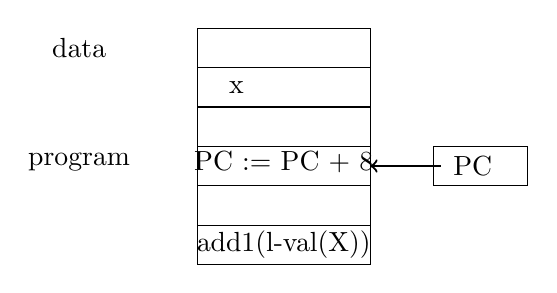
\begin{tikzpicture}

\draw (0,-1.0)  rectangle (2.2,0.0);
\pgftext[at={\pgfpoint{1.1cm}{-0.75cm}}]{add1(l-val(X))} ;

\draw (0,-0.5)  rectangle (2.2,0.5);
\pgftext[at={\pgfpoint{0.65cm}{0.3cm}}]{} ;

\draw (0,0)  rectangle (2.2,0.5);
\pgftext[at={\pgfpoint{-1.5cm}{0.3cm}}]{program} ;
\pgftext[at={\pgfpoint{1.1cm}{0.3cm}}]{PC := PC + 8} ;



\draw (0,0.5)  rectangle (2.2,1.0);
\pgftext[at={\pgfpoint{0.5cm}{0.75cm}}]{} ;


\draw(0,1.0)  rectangle (2.2,1.5);
\pgftext[at={\pgfpoint{0.5cm}{1.25cm}}]{x} ;


\draw (0,1.5)  rectangle (2.2,2.0);
\pgftext[at={\pgfpoint{-1.5cm}{1.75cm}}]{data} ;


% right one 
\draw (3,0)  rectangle (4.2,0.5);
\pgftext[at={\pgfpoint{3.5cm}{0.25cm}}]{PC} ;
\draw[<-, thick] (2.2,0.25) -- (3.1,0.25); 
%
\end{tikzpicture}
}
\end{tabular}
\end{tabular}


%\begin{center}
Imperative languages: also called 
\textit{von Neumann languages.} 
%\end{center}
\end{frame}


\begin{frame}[fragile]
\frametitle{An example in Fortran}
\framesubtitle{}

%Webber, p.185
\begin{cplus3}
    FUNCTION AVG(ARR,N)
    DIMENSION ARR(N)
    SUM = 0.0
    DO I = 1,N
       SUM = SUM + ARR(I)
    END DO
    AVG = SUM /FLOAT(N)
    RETURN 
    END FUNCTION
\end{cplus3}
\end{frame}

\mycomment{
\begin{frame}[fragile]
\frametitle{An example in COBOL}
\url{http://www.engin.umd.umich.edu/CIS/course.des/cis400/cobol/seccob.html}

\begin{cplus3}

000100 ID DIVISION.
000200 PROGRAM-ID.  ACCEPT1.
000300 DATA DIVISION.
000400 WORKING-STORAGE  SECTION.
000500 01  WS-FIRST-NUMBER      PIC 9(3).
000600 01  WS-SECOND-NUMBER     PIC 9(3).
000700 01  WS-TOTAL             PIC ZZZ9.
000800*
000900 PROCEDURE DIVISION.
001000 0000-MAINLINE.
001100     DISPLAY 'ENTER A NUMBER: '.
001200     ACCEPT WS-FIRST-NUMBER.
001300*
001400     DISPLAY 'ANOTHER NUMBER: '.
001500     ACCEPT WS-SECOND-NUMBER.
001600*
001700     COMPUTE WS-TOTAL = WS-FIRST-NUMBER + WS-SECOND-NUMBER.
001800     DISPLAY 'THE TOTAL IS: ', WS-TOTAL.
001900     STOP RUN.
\end{cplus3}
\end{frame}
}

\begin{frame}[fragile]
\frametitle{An example in Algol}
\url{http://www.engin.umd.umich.edu/CIS/course.des/cis400/algol/average.html}
\begin{cplus3}
// the main program (this is a comment)
begin
  integer N;
  Read Int(N);

  begin
    real array Data[1:N];
    real sum, avg;
    integer i;
    sum:=0;

    for i:=1 step 1 until N do
      begin real val;
        Read Real(val);
        Data[i]:=if val<0 then -val else val
      end;

    for i:=1 step 1 until N do
      sum:=sum + Data[i];
    avg:=sum/N;
    Print Real(avg)
  end
end	
\end{cplus3}
\end{frame}



\begin{frame}[fragile]
\frametitle{Key concepts}
\framesubtitle{}
\begin{itemize}
\item Variables
\item Procedures
\item (Commands)
\item (Data types)
\end{itemize}
\end{frame}



\section{Variables}
\begin{frame}[fragile]
\frametitle{Attributes of variables }
\framesubtitle{}
``Once a programmer has understood the use of variables, he has
understood the essence of programming.'' (Dijkstra)
\bigskip

Variables are bound to memory.

\begin{itemize}
\item What?
\begin{itemize}
\item l-value vs.r-value; copy vs. reference
\end{itemize}
\item How long?

\begin{itemize}
\item Lifetime 
\end{itemize}
\item Where? 
\begin{itemize}
\item Activation record, run-time stack vs. heap vs. static area
\end{itemize}
\end{itemize}
\end{frame}

\subsection{L-values and R-values}
\begin{frame}[fragile]
\frametitle{Storage model}
\framesubtitle{}
An abstract store is a collection of cells. A cell is either 
\textit{allocated} or not
allocated, its content is either defined or undefined.

{\small 
\center
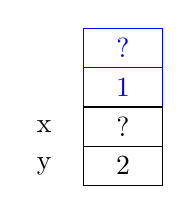
\begin{tikzpicture}

\tikzstyle{cell}=[rectangle,draw,minimum width=1cm,minimum height=0.5cm]

\draw[blue] ( 0,2) node [cell] {?} ;
\draw[blue] ( 0,1.5) node [cell] {1} ;
\draw (-1,1) node {x} ;
\draw ( 0,1) node [cell] {?} ;
\draw (-1,0.5) node {y} ;
\draw ( 0,0.5) node [cell] {2} ;



\end{tikzpicture}
}



\mycomment{

\bigskip
 
Simple vs.compound: 
\bigskip 

\begin{tabular}{ll}

\begin{minipage}{6cm}
\begin{itemize}
\item Simple (primitive):
    \\ contains one storable value
\item Compound: 
\\ contains multiple, contiguously
stored storable value
\end{itemize}

\end{minipage}
& 
\begin{tabular}{l}
{\small 
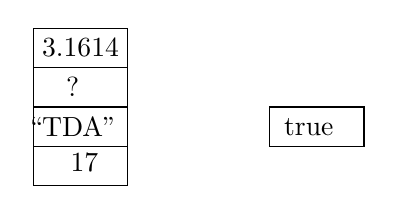
\begin{tikzpicture}
\draw (0,0)  rectangle (1.2,0.5);
\pgftext[at={\pgfpoint{0.65cm}{0.3cm}}]{17} ;

\draw (0,0.5)  rectangle (1.2,1.0);
\pgftext[at={\pgfpoint{0.5cm}{0.75cm}}]{``TDA''} ;



\draw (0,1.0)  rectangle (1.2,1.5);
\pgftext[at={\pgfpoint{0.5cm}{1.25cm}}]{?} ;

\draw (0,1.5)  rectangle (1.2,2.0);
\pgftext[at={\pgfpoint{0.6cm}{1.75cm}}]{3.1614} ;


\draw (3.0,0.5)  rectangle (4.2,1.0);
\pgftext[at={\pgfpoint{3.5cm}{0.75cm}}]{true} ;

\end{tikzpicture}
}
\end{tabular}
\end{tabular}

}


\end{frame}


\begin{frame}[fragile]
\frametitle{Example (storage model)}
\framesubtitle{}
% Watt, p.59
\begin{tabular}{ll}
\begin{minipage}{4cm}
\begin{cplus3}
/* A block in C */
{
   int n;
   n = 0;
   n = n+ 1;
}
\end{cplus3}
\end{minipage}
& 
\begin{tabular}{l}
{\small 
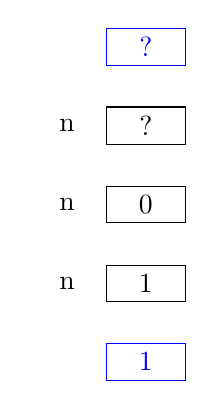
\begin{tikzpicture}

\draw[blue] ( 0,2)     node [rectangle, draw,minimum width=1cm] {?} ;

\draw (-1,1)     node [minimum width=1cm]                 {n} ;
\draw ( 0,1)     node [rectangle, draw,minimum width=1cm] {?} ;


\draw (-1,0)     node [minimum width=1cm]                 {n} ;
\draw ( 0,0)     node [rectangle, draw,minimum width=1cm] {0} ;


\draw (-1,-1.0)     node [minimum width=1cm]                 {n} ;
\draw ( 0,-1.0)     node [rectangle, draw,minimum width=1cm] {1} ;

\draw[blue] ( 0,-2)     node [rectangle, draw,minimum width=1cm] {1} ;


\end{tikzpicture}
}
\end{tabular}
\end{tabular}
\end{frame}

\begin{frame}[fragile]
\frametitle{L-values and R-values}
\framesubtitle{}
In any von Neumann language, a variable is (both)
\begin{itemize} 
    \item A memory location                 (if used on the left of :=)
    \item The value stored at such location  (if used on the right of :=)
\end{itemize}

Example:
\begin{cplus3}
     x := x + 1;
\end{cplus3}

The notion can be generalized to expressions (C, \cpp, ...):
\begin{itemize}
\item an expression is an l-value $\Leftrightarrow$ it can be used on the left of :=
% \item Some languages have a different syntax for l-values 
\item (sometimes): r-value: expression which is not an l-value
%
\mycomment{
\begin{itemize}
\item Exception: ML
\begin{cplus3}
- val myvar = ref 1;
val myvar = ref 1 : int ref
- !myvar;
val it = 1 : int
- myvar := 2;
val it = () : unit
- !myvar;
val it = 2 : int

\end{cplus3}
\end{itemize}
}
\item Most languages prevent observation of the address of an l-value
\begin{itemize}
\item Exception: the address-of operator in C/\cpp
\begin{cplus3}
  x = &y;
\end{cplus3}
\end{itemize}
\end{itemize}


\end{frame}



\begin{frame}
\frametitle{Copy semantics and reference semantics}
\framesubtitle{Semantics of assignment}
Assume:
{\small 
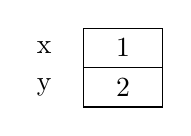
\begin{tikzpicture}

\tikzstyle{cell}=[rectangle,draw,minimum width=1cm,minimum height=0.5cm]

\draw (-1,1) node {x} ;
\draw ( 0,1) node [cell] {1} ;
\draw (-1,0.5) node {y} ;
\draw ( 0,0.5) node [cell] {2} ;



\end{tikzpicture}
}and consider the assignment $    x : = y; $


\begin{itemize}
\item Copy semantics:  the contents of $y$ are copied to $x$.
{\small 
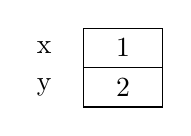
\begin{tikzpicture}

\tikzstyle{cell}=[rectangle,draw,minimum width=1cm,minimum height=0.5cm]

\draw (-1,1) node {x} ;
\draw ( 0,1) node [cell] {1} ;
\draw (-1,0.5) node {y} ;
\draw ( 0,0.5) node [cell] {2} ;



\end{tikzpicture}
}
\item Reference semantics: use location of $y$ as the location for $x$.
(They become \textit{aliases} of one another)
{\small 
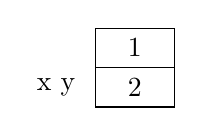
\begin{tikzpicture}

\tikzstyle{cell}=[rectangle,draw,minimum width=1cm,minimum height=0.5cm]

\draw ( 0,1) node [cell] {1} ;
\draw (-1,0.5) node {x y} ;
\draw ( 0,0.5) node [cell] {2} ;



\end{tikzpicture}
}

\end{itemize}
\end{frame}


\begin{frame}
\frametitle{Reference semantics, take 2.}
\framesubtitle{Explicit references in the storage model.}

One can also make references explicitly in the model (as arrows here.)

{\small 
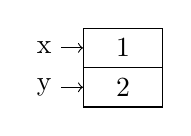
\begin{tikzpicture}

\tikzstyle{cell}=[rectangle,draw,minimum width=1cm,minimum height=0.5cm]

\node       (x)  at  (-1,1) {x} ;
\node[cell] (c1) at  ( 0,1) {1} ;
\node       (y)  at (-1,0.5) {y} ;
\node[cell] (c2) at (0,0.5) {2} ;
\draw [->] (x) -- (c1);
\draw [->] (y) -- (c2);

\end{tikzpicture}
}
$x := y;$
{\small 
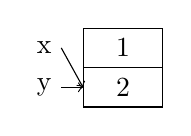
\begin{tikzpicture}

\tikzstyle{cell}=[rectangle,draw,minimum width=1cm,minimum height=0.5cm]

\node       (x)  at  (-1,1) {x} ;
\node[cell] (c1) at  ( 0,1) {1} ;
\node       (y)  at (-1,0.5) {y} ;
\node[cell] (c2) at (0,0.5) {2} ;
\draw [->] (x.east) -- (c2.west);
\draw [->] (y) -- (c2);

\end{tikzpicture}
}

You can think of the assignment as ``the reference is copied''.

\end{frame}




\begin{frame}[fragile]
\frametitle{Copy semantics in \Cpp}
\framesubtitle{}
% Watt, p.64
Assignments in \Cpp 
\begin{itemize}
\item \Cpp supports copy semantics only. 
\item Developers can achieve the
effect of reference semantics by using pointers. 
\end{itemize}

\begin{cplus}
class date {
private:
    int y, m, d;
public:
    date(int y, int m, int d) {..}
    date() {}
};

date today = date(2007,10,30);
date tomorrow; 
tomorrow = today;  // copy semantics

// pointers achieve the effect of reference semantics
date* another_pointer = new date(2007,12,10);
date* tomorrow_ptr    = another_ptr;   // aliasing
*tomorrow__ptr = today;
\end{cplus}


\end{frame}

\begin{frame}[fragile]
\frametitle{Reference semantics in Java}
\framesubtitle{}
% XXX Should be the same with C\#
% Watt, p.64
Java distinguishes two kinds of assignments 
\begin{itemize}
\item Java supports reference semantics for objects and copy semantics
for primitive values.
\item Developers can achieve the effect of copy semantics by using
the (appropriately implemented) \textit{clone()} method.
\end{itemize}

\begin{java}
class Date 
{
    int y, m, d;
    public Date(int y, int m, int d) {..}
}

Date today    = new Date(2007,10,30);
Date tomorrow = new Date(2007,10,31);
today = tomorrow;    // reference semantics

// copy semantics 
Date date1 = today.clone();
\end{java}
%pics
\end{frame}



\begin{frame}[fragile]
\frametitle{Equality}
\framesubtitle{}
The semantics of the equality predicate should be consistent with
the semantics of the assignment (why?).

Assume 
\begin{cplus3}
          if (...) { x := y; } 
          ...
          if (x == y) ... 
\end{cplus3}
\begin{itemize}
\item Copy semantics: test whether the corresponding components contain
the same values.
\item Reference semantics: test whether $x,y$ are aliases (i.e., point
to the same address). 
\end{itemize}
\end{frame}

\mycomment{
\begin{frame}[fragile]
\frametitle{Equality on reference types in C\#}
\framesubtitle{}
Equality (and cloning) are easy to get wrong.

\begin{itemize}
\item \texttt{o1 == o2}
\begin{itemize}
\item true if o1, o2 are null or created by the same \texttt{new}. Can be overloaded.
\end{itemize}

\item \texttt{o1.Equals(o2)}
\begin{itemize}
\item true if o1, o2  created by the same \texttt{new}. Can be overridden. 
\end{itemize}

\item \texttt{Object.ReferenceEquals(o1,o2)}
\begin{itemize}
\item true if o1, o2 are null or created by the same \texttt{new}.
\end{itemize}

\item \texttt{Object.Equals(o2)}
\begin{itemize}
\item true if Object.ReferenceEquals(o1,o2) or o1.Equals(o2).
\end{itemize}
\end{itemize}

\end{frame}
}


\subsection{Lifetime and storage classes}
\begin{frame}[fragile]
\frametitle{Lifetime} 
\framesubtitle{}
The \textit{lifetime} (``extent'') of a variable is the time during which it is
bound to memory, i.e., the time between allocation and deallocation.
\bigskip

Each variable has a storage class. 
Storage classes classify variables according to their lifetime.
\begin{itemize}
\item Global: live throughout the program
\item Local:  during the ``activation'' of its block
\item Heap: no general rule, until deallocated (manually or automatically) 
%\item Persistent: beyond the execution of the program
\end{itemize}

\end{frame}

\begin{frame}[fragile]
\frametitle{Global variables}
\framesubtitle{}
A global variable is allocated and initialized at program start and deallocated
at program end. No re-initialization in between.

\bigskip
In C, static variables and variables in ``global scope''  are global:
\begin{cplus3}
/* global variables in C */
int count = 0;
int nextcount() {
    count++;
    return count;
}

/* static variables in C */
int nextcount() {
    static int count = 0;
    count++;
    return count;
}
\end{cplus3}
\end{frame}


\begin{frame}[fragile]
\frametitle{Local variables}
\framesubtitle{}
A local variable is declared in a block and can be used only
within this block.
\begin{itemize}
\item Allocated at the beginning of the block.
\item Deallocated at the end of the block.
\end{itemize}

\begin{cplus3}
   { 
       int x;
       double f;
       ...

   }
\end{cplus3}
\bigskip

\textit{Activation} of a block: the time during which the block executes.
\begin{itemize}
\item In case of procedure: the time between call and return.
\end{itemize}
A block can be activated several times in a program (how?)\\  $\leadsto$
a local variable can have several lifetimes.  
\end{frame}

\begin{frame}[fragile]
\frametitle{Heap variables}
\framesubtitle{}
A heap variable can be allocated and deallocated at arbitrary times in
the program.
\begin{itemize}
\item Allocated and initialized at run time and explicitly, 
via an expression, e.g., \texttt{malloc, new}.
% Compare to local: by declaration
\item The variable itself is anonymous and accessible only through 
 a pointer or reference. 
\item Deallocation: when the variable is no longer ``reachable.''
Either manually (\texttt{delete}) or through garbage collection. 
\end{itemize}
\end{frame}

\begin{frame}
\frametitle{Multiple storage classes} 
% If a language supports more than one storage class, two major decisions are necessary:
Major decisions:
\begin{itemize}

\item Built-in types: should users control the storage class of a
variable of built-in type?
\begin{itemize}
\item If yes: how? If no: language specification needed.
\end{itemize}

\item User-defined types: should users control the storage class of 
``their'' type?
\begin{itemize}
\item If yes: how? If no: language specification needed.
\end{itemize}

\end{itemize}

Examples:
\begin{itemize}
\item In Fortran77, one storage class only; all variables are global.
\item 
In \Cpp, all three storage classes are supported; the user
specifies which one to use. 
\item In Java/C\#, all three storage classes are supported, but the
user cannot fully control. 
\end{itemize}
% Q: What decisions were taken in Java? 
% xxx Can one write Integer j = new int(i)?
\mycomment{Final in Java?}
\end{frame}



\subsection{The Need for A Stack}
\begin{frame}[fragile]
\frametitle{Activation records}
\framesubtitle{}
% Webb, p.184
Activations:
\begin{itemize}
\item A function can have different \textit{activations} during the
execution of a program (multiple callers).
\item Multiple activations
can be alive at a time (call chain).
\end{itemize}

\begin{cplus3}
    main()  {
         beta();
         ...
         alpha(i);
    }
    beta(){
         ... 
         alpha(j);
    }
\end{cplus3}



\bigskip

\textit{Activation record} (AR): stores activation-specific information
\begin{itemize}
\item Return address
\item (Local) variables
\item \ldots and more (see below)
\end{itemize}
%Layout of AR:  important design decision for run-time system. 
\end{frame}

\begin{frame}[fragile]
\frametitle{Static allocation of activation records}
\framesubtitle{}
Static allocation is simple:
\begin{itemize}
\item Allocate one AR per function, at compile time.

\item Example (Fortran)



\begin{tabular}{ll}

\begin{minipage}{6cm}

\begin{cplus3}
    FUNCTION AVG(ARR,N)
    DIMENSION ARR(N)
    SUM = 0.0
    DO I = 1,N
       SUM = SUM + ARR(I)
    END DO
    AVG = SUM /FLOAT(N)
    RETURN 
    END FUNCTION 
\end{cplus3}

\end{minipage}
& 
\begin{minipage}{6cm}
{\small 
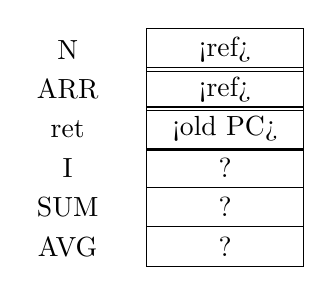
\begin{tikzpicture}

\tikzstyle{cell}=[rectangle,draw,minimum width=2cm,minimum height=0.5cm]

\node       (N)   at  (-2,  1) {N} ;
\node       (ARR) at  (-2,0.5) {ARR} ;
\node       (ret) at  (-2,  0) {ret} ;
\node       (I)   at  (-2,-.5) {I} ;
\node       (SUM) at  (-2, -1) {SUM} ;
\node       (AVG) at  (-2,-1.5) {AVG} ;

\node[cell] (c1) at (0,1) {<ref>} ;
\node[cell] (c2) at (0,0.5) {<ref>} ;
\node[cell] (c2) at (0,0)   {<old PC>} ;
\node[cell] (c2) at (0,-.5)   {?} ;
\node[cell] (c2) at (0,-1)   {?} ;
\node[cell] (c2) at (0,-1.5)   {?} ;

% \draw [->] (x) -- (c1);
% \draw [->] (y) -- (c2);


\end{tikzpicture}
}
\end{minipage}
\end{tabular}
\end{itemize}

Assumptions:
\begin{itemize}
\item All (size) information available statically
\item No more than one activation of a function alive
at the same time
\end{itemize}
Q: when are those assumptions not valid?

\end{frame}

\begin{frame}[fragile]
\frametitle{Dynamic chain of activation records}

Languages that support recursion must provide one AR per
activation of a function (\emph{not} per function).

\begin{itemize}
\item ARs must be allocated dynamically.
\begin{itemize}
\item When the function is called, a new AR is allocated.
\item When the function returns, its AR released.
\end{itemize}
\item AR must include additional information, to enable the dynamic
allocation (of ARs): 
\begin{itemize}
\item Address of previous AR (why?)
\end{itemize}
\end{itemize}
\end{frame}

\begin{frame}
\frametitle{The Stack}


\begin{itemize}
\item In typical imperative languages, ARs are allocated LIFO. (Why?)
\item An easy way to implement allocation/deallocation is to use a \emph{stack}.
\end{itemize}

In such a context:
\begin{itemize}

\item ARs are sometimes called \textit{stack frames}. 

\item The computer architecture may support this natively. (Hence ``The System Stack'')

\item Do you still need address of previous AR?

\end{itemize}

The rest of the lecture assumes a LIFO allocation policy.

\end{frame}

\begin{frame}[fragile]
\frametitle{Example}
\framesubtitle{Dynamic allocation of activation records}
Snapshot  of the recursive function
 \texttt{fact}, at  \texttt{fact(3)}, before 
\texttt{fact(2)} has been
called.
\bigskip



\begin{tabular}{ll}
\begin{minipage}{6cm}
\begin{cplus3}
int fact(int n) {
   int result;
   if (n<2) result = 1;
   else result = n * fact(n-1);
   return result;
}
\end{cplus3}
\end{minipage}
& 
\begin{tabular}{l}
{\small 
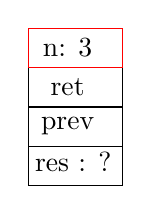
\begin{tikzpicture}
\draw (0,0)  rectangle (1.2,0.5);
\pgftext[at={\pgfpoint{0.65cm}{0.3cm}}]{res : ? } ;

\draw (0,0.5)  rectangle (1.2,1.0);
\pgftext[at={\pgfpoint{0.5cm}{0.75cm}}]{prev} ;



\draw (0,1.0)  rectangle (1.2,1.5);
\pgftext[at={\pgfpoint{0.5cm}{1.25cm}}]{ret} ;

\draw[red] (0,1.5)  rectangle (1.2,2.0);
\pgftext[at={\pgfpoint{0.5cm}{1.75cm}}]{n: 3} ;

\end{tikzpicture}
}
\end{tabular}
\end{tabular}
\begin{itemize}
\item Local variable $n$: value 3.
\item Ret: holds the address of the instruction to execute
after \texttt{fact(3)} has returned.
\item Prev: holds the address of the caller's AR. 
\item Res: not initialized.
\end{itemize}
\end{frame}

\begin{frame}[fragile]
\frametitle{Example (cont'd)}
\framesubtitle{}
Second activation of \texttt{fact},
at  \texttt{fact(2)}, before 
\texttt{fact(1)} has been
called. 
 First AR still present, but execution is suspended
(until second activation returns).
\bigskip

\begin{tabular}{ll}
\begin{minipage}{6.5cm}
%
Second AR:

\begin{itemize}
\item Local variable $n$: holds value 2.
\item Ret: holds the address of the instruction to execute after 
\texttt{fact(2)} has returned.
\item Prev: holds the address of first AR;  note that the run-time stack grows to the left. 
\item Res: not initialized.
\end{itemize}
\end{minipage}
& 
\begin{tabular}{l}
{\small 
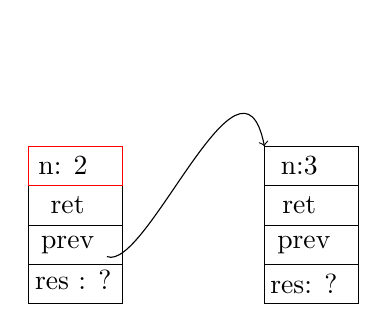
\begin{tikzpicture}
\draw (0,0)  rectangle (1.2,0.5);
\pgftext[at={\pgfpoint{0.65cm}{0.3cm}}]{res : ? } ;

\draw (0,0.5)  rectangle (1.2,1.0);
\pgftext[at={\pgfpoint{0.5cm}{0.75cm}}]{prev} ;
\draw[->] (1.0, 0.6) .. controls (1.5, 0.4) and (2.7, 3.5) .. (3,2.0);


\draw (0,1.0)  rectangle (1.2,1.5);
\pgftext[at={\pgfpoint{0.5cm}{1.25cm}}]{ret} ;

\draw[red] (0,1.5)  rectangle (1.2,2.0);
\pgftext[at={\pgfpoint{0.5cm}{1.75cm}}]{n: 2 } ;

%\draw[red] (0,2.0)  rectangle (1.2,2.5);
%\pgftext[at={\pgfpoint{0.5cm}{2.25cm}}]{a: 3 } ;

% right one 
\draw (3,0)  rectangle (4.2,0.5);
\pgftext[at={\pgfpoint{3.5cm}{0.25cm}}]{res: ?} ;

\draw (3,0.5)  rectangle (4.2,1.0);
\pgftext[at={\pgfpoint{3.5cm}{0.75cm}}]{prev} ;

\draw (3,1.0)  rectangle (4.2,1.5);
\pgftext[at={\pgfpoint{3.5cm}{1.25cm}}]{ret } ;

\draw (3,1.5)  rectangle (4.2,2.0);
\pgftext[at={\pgfpoint{3.5cm}{1.75cm}}]{n:3 } ;

\end{tikzpicture}
}
\end{tabular}
\end{tabular}
\end{frame}


\begin{frame}[fragile]
\frametitle{Example (cont'd)}
\framesubtitle{}
Third activation of \texttt{fact},
at  \texttt{fact(1)}, just before 
returning to its caller. 

\begin{itemize}
\item The variable $res$ is initialized. 
\item No further recursion.
\end{itemize}


\begin{tabular}{ll}
\begin{minipage}{4cm}

\end{minipage}
& 
\begin{tabular}{l}
{\small 
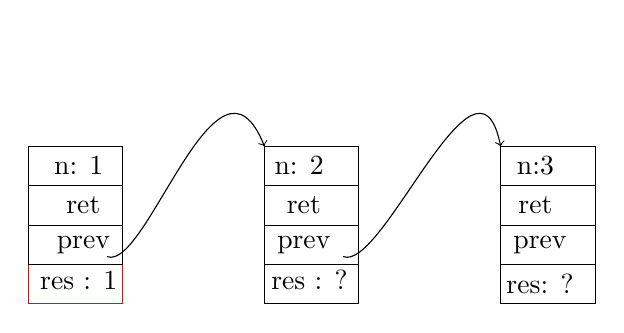
\begin{tikzpicture}

%left one
\draw[red] (-3.0,0)  rectangle (-1.8,0.5);
\pgftext[at={\pgfpoint{-2.3cm}{0.3cm}}]{res : 1 } ;

\draw (-3.0,0.5)  rectangle (-1.8,1.0);
\pgftext[at={\pgfpoint{-2.3cm}{0.75cm}}]{prev} ;
\draw[->] (-2.0, 0.6) .. controls (-1.5, 0.4) and (-0.6, 3.5) .. (0,2.0);


\draw (-3.00,1.0)  rectangle (-1.8,1.5);
\pgftext[at={\pgfpoint{-2.3cm}{1.25cm}}]{ret} ;

\draw (-3.0,1.5)  rectangle (-1.8,2.0);
\pgftext[at={\pgfpoint{-2.3cm}{1.75cm}}]{n: 1 } ;

% middle one

\draw (0,0)  rectangle (1.2,0.5);
\pgftext[at={\pgfpoint{0.65cm}{0.3cm}}]{res : ? } ;

\draw (0,0.5)  rectangle (1.2,1.0);
\pgftext[at={\pgfpoint{0.5cm}{0.75cm}}]{prev} ;
\draw[->] (1.0, 0.6) .. controls (1.5, 0.4) and (2.7, 3.5) .. (3,2.0);


\draw (0,1.0)  rectangle (1.2,1.5);
\pgftext[at={\pgfpoint{0.5cm}{1.25cm}}]{ret} ;

\draw (0,1.5)  rectangle (1.2,2.0);
\pgftext[at={\pgfpoint{0.5cm}{1.75cm}}]{n: 2 } ;


% right one 
\draw (3,0)  rectangle (4.2,0.5);
\pgftext[at={\pgfpoint{3.5cm}{0.25cm}}]{res: ?} ;

\draw (3,0.5)  rectangle (4.2,1.0);
\pgftext[at={\pgfpoint{3.5cm}{0.75cm}}]{prev} ;

\draw (3,1.0)  rectangle (4.2,1.5);
\pgftext[at={\pgfpoint{3.5cm}{1.25cm}}]{ret } ;

\draw (3,1.5)  rectangle (4.2,2.0);
\pgftext[at={\pgfpoint{3.5cm}{1.75cm}}]{n:3 } ;

\end{tikzpicture}
}
\end{tabular}
\end{tabular}

\end{frame}


\begin{frame}[fragile]
\frametitle{Example (cont'd)}
\framesubtitle{}
Snapshot of run-time stack, just before the
second activation returns:

\begin{itemize}
\item The second AR gets the value 1 from \texttt{fact(1)}
and the variable $res$ is set to $2\times 1 = 2$.
\item The activation record for the third activation is
popped off the run-time stack. 
\end{itemize}


\begin{tabular}{ll}
\begin{minipage}{4cm}

\end{minipage}
& 
\begin{tabular}{l}
{\small 
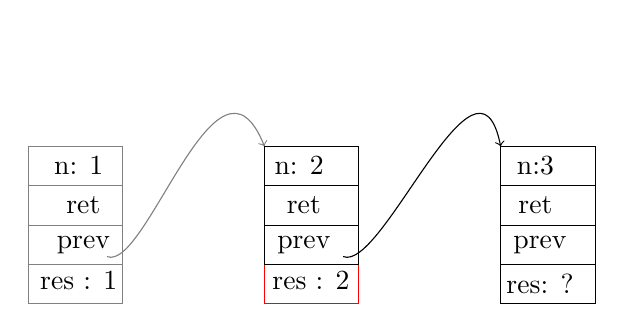
\begin{tikzpicture}

%left one
\draw[gray] (-3.0,0)  rectangle (-1.8,0.5);
\pgftext[at={\pgfpoint{-2.3cm}{0.3cm}}]{res : 1 } ;

\draw[gray] (-3.0,0.5)  rectangle (-1.8,1.0);
\pgftext[at={\pgfpoint{-2.3cm}{0.75cm}}]{prev} ;
\draw[gray,->] (-2.0, 0.6) .. controls (-1.5, 0.4) and (-0.6, 3.5) .. (0,2.0);


\draw[gray] (-3.00,1.0)  rectangle (-1.8,1.5);
\pgftext[at={\pgfpoint{-2.3cm}{1.25cm}}]{ret} ;

\draw[gray] (-3.0,1.5)  rectangle (-1.8,2.0);
\pgftext[at={\pgfpoint{-2.3cm}{1.75cm}}]{n: 1 } ;

% middle one

\draw[red] (0,0)  rectangle (1.2,0.5);
\pgftext[at={\pgfpoint{0.65cm}{0.3cm}}]{res : 2 } ;

\draw (0,0.5)  rectangle (1.2,1.0);
\pgftext[at={\pgfpoint{0.5cm}{0.75cm}}]{prev} ;
\draw[->] (1.0, 0.6) .. controls (1.5, 0.4) and (2.7, 3.5) .. (3,2.0);


\draw (0,1.0)  rectangle (1.2,1.5);
\pgftext[at={\pgfpoint{0.5cm}{1.25cm}}]{ret} ;

\draw (0,1.5)  rectangle (1.2,2.0);
\pgftext[at={\pgfpoint{0.5cm}{1.75cm}}]{n: 2 } ;

%\draw[red] (0,2.0)  rectangle (1.2,2.5);
%\pgftext[at={\pgfpoint{0.5cm}{2.25cm}}]{a: 3 } ;

% right one 
\draw (3,0)  rectangle (4.2,0.5);
\pgftext[at={\pgfpoint{3.5cm}{0.25cm}}]{res: ?} ;

\draw (3,0.5)  rectangle (4.2,1.0);
\pgftext[at={\pgfpoint{3.5cm}{0.75cm}}]{prev} ;

\draw (3,1.0)  rectangle (4.2,1.5);
\pgftext[at={\pgfpoint{3.5cm}{1.25cm}}]{ret } ;

\draw (3,1.5)  rectangle (4.2,2.0);
\pgftext[at={\pgfpoint{3.5cm}{1.75cm}}]{n:3 } ;


\end{tikzpicture}
}
\end{tabular}
\end{tabular}

\end{frame}

\begin{frame}[fragile]
\frametitle{Example (cont'd)}
\framesubtitle{}
Snapshot of run-time stack, just before the
first activation returns:

\begin{itemize}
\item The first AR gets the value 2 from \texttt{fact(2)}
and the variable $res$ is set to $3\times 2 = 6$.
\item The activation record for the second activation is
popped off the run-time stack. 
\end{itemize}

\begin{tabular}{ll}
\begin{minipage}{4cm}

\end{minipage}
& 
\begin{tabular}{l}
{\small 
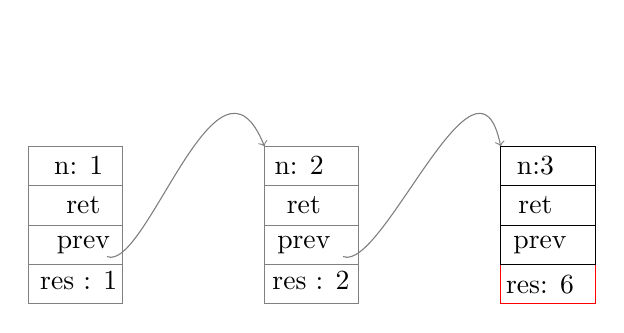
\begin{tikzpicture}

%left one
\draw[gray] (-3.0,0)  rectangle (-1.8,0.5);
\pgftext[at={\pgfpoint{-2.3cm}{0.3cm}}]{res : 1 } ;

\draw[gray] (-3.0,0.5)  rectangle (-1.8,1.0);
\pgftext[at={\pgfpoint{-2.3cm}{0.75cm}}]{prev} ;
\draw[gray,->] (-2.0, 0.6) .. controls (-1.5, 0.4) and (-0.6, 3.5) .. (0,2.0);


\draw[gray] (-3.00,1.0)  rectangle (-1.8,1.5);
\pgftext[at={\pgfpoint{-2.3cm}{1.25cm}}]{ret} ;

\draw[gray] (-3.0,1.5)  rectangle (-1.8,2.0);
\pgftext[at={\pgfpoint{-2.3cm}{1.75cm}}]{n: 1 } ;

% middle one

\draw[gray] (0,0)  rectangle (1.2,0.5);
\pgftext[at={\pgfpoint{0.65cm}{0.3cm}}]{res : 2 } ;

\draw[gray] (0,0.5)  rectangle (1.2,1.0);
\pgftext[at={\pgfpoint{0.5cm}{0.75cm}}]{prev} ;
\draw[gray,->] (1.0, 0.6) .. controls (1.5, 0.4) and (2.7, 3.5) .. (3,2.0);


\draw[gray] (0,1.0)  rectangle (1.2,1.5);
\pgftext[at={\pgfpoint{0.5cm}{1.25cm}}]{ret} ;

\draw[gray] (0,1.5)  rectangle (1.2,2.0);
\pgftext[at={\pgfpoint{0.5cm}{1.75cm}}]{n: 2 } ;



% right one 
\draw[red] (3,0)  rectangle (4.2,0.5);
\pgftext[at={\pgfpoint{3.5cm}{0.25cm}}]{res: 6} ;

\draw (3,0.5)  rectangle (4.2,1.0);
\pgftext[at={\pgfpoint{3.5cm}{0.75cm}}]{prev} ;

\draw (3,1.0)  rectangle (4.2,1.5);
\pgftext[at={\pgfpoint{3.5cm}{1.25cm}}]{ret } ;

\draw (3,1.5)  rectangle (4.2,2.0);
\pgftext[at={\pgfpoint{3.5cm}{1.75cm}}]{n:3 } ;


\end{tikzpicture}
}
\end{tabular}
\end{tabular}

\end{frame}




\mycomment{

Stack-based language now refer to Forth, and so on.

\begin{frame}[fragile]
\frametitle{Stack-based languages}
Languages where ARs are allocated and deallocated in a
stack-based fashion, are called \textit{stack-based languages}. 

\begin{itemize}
\item Big class of languages
\begin{itemize}
\item  All languages mentioned so far 
(Algol, C, Java, \Cpp, C\#, Ada, Pascal, COBOL, \ldots)
\end{itemize}
\item For stack-based languages with nested functions and non-local references,
the AR must be extended:
\begin{itemize}
\item  Include a pointer  (``static link'') to the AR of the enclosing function,
i.e., the static parent 
\item Ada, Pascal (but \textit{not}: C, Java, \Cpp, C\#)
\end{itemize}

\begin{cplus3}
int x,y,z;
f1() {
   int a,b;
   f2() {
       int x;w;
       f3() {
          int y,w,a;
       }
       x = y + t + w + z; }}
\end{cplus3}
\end{itemize}

\end{frame}

}

\mycomment {

I think the below is confusing: one may keep references to AR even in imperative lang. like C.
(The runtime will just be reckless an deallocate anyway!)

\begin{frame}[fragile]
\frametitle{Functions as parameters}
In \textit{functional} languages, functions are first-class
citizens and can be passed and returned as any other variable.

\begin{itemize}
\item Static link does not suffice; may need to keep the implementation.
\item References into ARs may exist even if the function
has returned.
% Webb 202
\item Stack-based allocation discipline no longer possible.

\end{itemize}

\end{frame}

}

\begin{frame}[fragile]
\frametitle{Organization of memory}
\framesubtitle{Block-structured languages}
A program can hold its data in different segments of memory.
\begin{itemize}
\item Static area for global variables
\begin{itemize}
\item Fixed size (``static'') for the duration of 
the program.
\end{itemize} 
\item (Run-time) stack for local variables (a.k.a. stack-based, automatic)
\begin{itemize}
\item  Grows and shrinks at run time in a disciplined
manner
\item  \emph{Activation records} are pushed and popped. 
\end{itemize}

\item Heap for heap-based variables
\begin{itemize}
\item Grows and possibly shrinks at run time but not
in a disciplined manner. 
\end{itemize}
\end{itemize}
Not every language supports all three kinds of memory; even if,
it might not give users control. 
\end{frame}


\begin{frame}[fragile]
\frametitle{Comparison}

{\small
\begin{tabular}{lcccc}
Region & Access        & Allocation policy & Allocation operation      & Comment \\
\hline 
Static & fixed address & At startup & Ask OS & Rigid and cheap \\
Stack  & AR + fixed address & LIFO & Bump stack pointer by fixed amount & Cheap (Local) \\
Heap   & Through any pointer & See below & See below & Flexible, but maybe expensive \\
\hline 
\end{tabular}
}

There are many representations for the Heap. Major distinction: GC or not.

Remark:Some language also have ``Bump stack pointer by dynamic amount'' allocation operation.

Exercise: work out the other column and think about the tradeoffs.

\end{frame}

\begin{frame}[fragile]
\frametitle{Evaluation (program design)}
\framesubtitle{}
What if the designer has a choice?
\bigskip

Decision criteria are lifetime, costs, and size.
\begin{itemize}
\item Does the compiler know the size of the variable at compile time?
\item Can the compiler initialize the variable at compile time?
\item Can the compiler allocate the variable at compile time?
\end{itemize}
\end{frame}



\mycomment{
\begin{frame}[fragile]
\frametitle{Pointers}
\framesubtitle{}
For a pointer type, the value of an instance is 
either a location in memory or a special
value (e.g., null). 
\bigskip

Why pointers? 
\begin{itemize}
\item Heap-based (anonymous) variables 
\begin{cplus3}
char* cp;
Date d = new Date();
\end{cplus3}
\item Recursive types (in imperative languages)
\begin{cplus3}
struct list_node {
    int element;
    struct list_node* next;
}
typedef struct list_node* list;
\end{cplus3}


\item Indirect addressing (assembly languages) 
%\begin{cplus3}
%\end{cplus3}
\end{itemize}

\end{frame}

\begin{frame}[fragile]
\frametitle{Recursive types}
\framesubtitle{}
Why are direct recursive types illegal in imperative languages?
\bigskip

\begin{tabular}{ll}
\begin{minipage}{4cm}

\begin{cplus3}
/* illegal in C */
union list {
    enum { nil } empty;
    struct {
       int element;
       union list next;   
    } list_node
}
\end{cplus3}
\end{minipage}

\begin{minipage}{7cm}
Recursive equation:
\begin{center}
   list = { nil} $\cup $ int $\times$ list
\end{center}
Theory shows: smallest solution (\textit{least fixed point})
exists:
\begin{center}
   {nil} $\cup$ int $\cup$ (char $\times$ char) $\cup$
   \\
  (char $\times$ char $\times$ char) $\cup$ \ldots
\end{center}
\end{minipage}
\end{tabular}

Recall:
\begin{itemize}
\item Stack-based variables must have a fixed size
\end{itemize}
\bigskip

Note that functional languages allow recursive types.
\begin{cplus3}
Haskell:
data List a = Nil | Cons a (List a)
\end{cplus3}

\mycomment {
ML
\begin{cplus3}
datatype MyList
    = Empty | MyListNode of int * MyList;
\end{cplus3}
}
\end{frame}

\begin{frame}[fragile]
\frametitle{Design questions}
\framesubtitle{}
Design 
\begin{itemize}
\item Lifetime
\begin{itemize}
\item Allocated by hand? Deallocated by hand?
\end{itemize}
\item Type
\begin{itemize}
\item (Implicit) conversions?
\begin{itemize}
\item int* to void*; child-ref to parent-ref, \ldots
\end{itemize}
\item Different from \ldots references? arrays?
\end{itemize}

\end{itemize}
\end{frame}


\begin{frame}[fragile]
\frametitle{Operations}

\begin{itemize}
\item Assignment
\begin{cplus3}
char* cp = another_pointer;
Date d = new Date();
Date d2 = new Date(5, 10);
d = d2;
\end{cplus3}

\item Dereferencing
\begin{cplus3}
int* ip = ptr_to_5;
int  i  = *ip;
\end{cplus3}

\item (Pointer arithmetic)
\begin{cplus3}
int iarray[10];
int* ip = iarray;
int j   = ip + 5;
\end{cplus3}

\end{itemize}
\end{frame}

\begin{frame}[fragile]
\frametitle{Classical problems} 
\framesubtitle{\ldots and how to cope with them}

Dangling pointers: r-value refers to deallocated variable
\begin{itemize}
\item Prohibit manual deallocation
\item Design small wrapper classes around pointers that manage shared ownership (aliasing)
\end{itemize}

Memory leakage: heap-based variable not reachable
\begin{itemize}
\item Automatic memory management (GC, destructors, finalizers)
\end{itemize}

Illegal access/out of bounds:
\begin{itemize}
\item Prohibit pointer arithmetic
\item Design fat pointer classes that include bounds checks (e.g., Java
iterators)
\item Bounded access as idiom 
\begin{cplus3}
// Standard Template Library in C++
list<int> L;
...
result = find(L.begin(), L.end(), 7);
\end{cplus3}
\end{itemize}


\end{frame}



\begin{frame}[fragile]
\frametitle{Implementation}
\framesubtitle{}
Simplest of all possible representations:
\begin{itemize}
\item Address: 2- or 4-byte (depending on address space)
\item Alternative: segment + offset
\end{itemize}
\end{frame}


} % end mycomment section pointers

\begin{frame}[fragile]
\frametitle{Summary}
Concepts discussed:
\bigskip

\begin{itemize}
\item L-value vs. r-value
\item Copy semantics vs. reference semantics
\item Storage classes and lifetime (global, local, heap)
\item Activation records (static and dynamic allocation), run-time stack,
static area and heap. 
\end{itemize}
\end{frame}


\section{Procedures}
\begin{frame}[fragile]
\frametitle{Terminology}
\framesubtitle{}

\begin{itemize}

\item Parameters
\begin{itemize}
\item Argument: the expression or value that is passed to the procedure
\item Actual parameter: the expression that yields the argument 
\item Formal parameter: the identifier in the method body 
\begin{cplus3}
int plus(int a, int b) {
   return a+b;
}
void f()  {
   int y = -5;
   int x = plus(1, abs(-5));
}
\end{cplus3}
Here: arguments are 1 and 5. Actual parameters: 1 and abs(-5). Formal
parameters: a and b. 
\end{itemize}
\item Distinguish: ``caller'' vs. callee''
\begin{itemize}
\item  In the example: \texttt{plus} is the callee, 
\texttt{f} the caller.
\end{itemize}
\end{itemize}


\end{frame}


\begin{frame}[fragile]
\frametitle{Design space}
\framesubtitle{Questions for language designers}
\begin{itemize}
\item What (= what attributes of the parameter) is passed during
procedure invocation? 

\begin{itemize}
\item Copy
\item Address
\item Name 
\end{itemize}
\item Direction of the information flow?
\begin{itemize}
\item Actual $\leadsto$ formal (caller $\leadsto$ callee)
\item Formal $\leadsto$ actual (callee $\leadsto$ caller)
\end{itemize}
\end{itemize}
\end{frame}

\begin{frame}[fragile]
\frametitle{Parameter passing mechanisms}
\begin{itemize}
\item Call-by-reference
\item Call-by-copy
\begin{itemize}
\item Call-by-value
\item Call-by-result
\item Call-by-value-result
\end{itemize}

\item Call by name: 

\begin{itemize}
\item Call-by-name
\item Call-by-need
\end{itemize}
\end{itemize}

Most languages support one or two mechanisms only. 
\begin{itemize}
\item More expressive:  C\#, \Cpp, Ada support several mechanisms.
\item Which mechanisms? See language specification. 
\item If users can select, keywords necessary (why?) 
\end{itemize}



\end{frame}

\begin{frame}[fragile]
\frametitle{Call-by-reference}
\begin{tabular}{ll}
\begin{minipage}{6cm}
\begin{cplus3}
void plus(int a, by-reference int b) {
    b = b + a;
}
void f() {
    int x = 3;
    plus(4,x);
}
\end{cplus3}
\end{minipage}

& 

\begin{tabular}{l}
{\small 
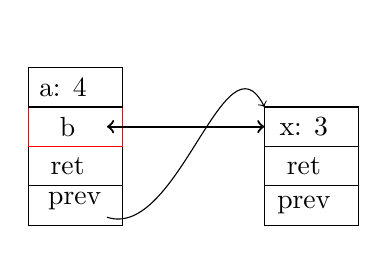
\begin{tikzpicture}
\draw (0,0)  rectangle (1.2,0.5);
\pgftext[at={\pgfpoint{0.65cm}{0.3cm}}]{prev } ;
\draw[->] (1.0, 0.1) .. controls (1.9, -0.2) and (2.5, 2.5) .. (3,1.5);

\draw (0,0.5)  rectangle (1.2,1.0);
\pgftext[at={\pgfpoint{0.5cm}{0.75cm}}]{ret} ;


\draw[red] (0,1.0)  rectangle (1.2,1.5);
\pgftext[at={\pgfpoint{0.5cm}{1.25cm}}]{b} ;
\draw[<->, thick] (1.0, 1.25) -- (3.0,1.25); 

\draw (0,1.5)  rectangle (1.2,2.0);
\pgftext[at={\pgfpoint{0.5cm}{1.75cm}}]{a: 4 } ;



% right one 
\draw (3,0)  rectangle (4.2,0.5);
\pgftext[at={\pgfpoint{3.5cm}{0.25cm}}]{prev} ;

\draw (3,0.5)  rectangle (4.2,1.0);
\pgftext[at={\pgfpoint{3.5cm}{0.75cm}}]{ret} ;

\draw (3,1.0)  rectangle (4.2,1.5);
\pgftext[at={\pgfpoint{3.5cm}{1.25cm}}]{x: 3} ;



\end{tikzpicture}
}
\end{tabular}
\end{tabular}
\begin{itemize}
\item The address of the actual parameter is passed.
Formal and actual parameter are aliases of another. 
\item Efficient (no copying of values). 
\item Unintended aliases have unintended effects. 
\end{itemize}
 Example: Fortran, ``\&''-parameter in \Cpp, ``ref'' parameter in C\#
\end{frame}


\begin{frame}[fragile]
\frametitle{Example: by-reference}
\framesubtitle{C\# and \Cpp}
In C\# 
\begin{itemize}
\item By-reference parameters are declared via ``ref.'' The modifier
is also necessary for the actual argument. 
\begin{cplus3}
class Arithmetics {
     static void SquareIt(ref int x) { x *= x;} }
}
int myInt = 5; SquareIt(ref myInt); 
\end{cplus3}
\end{itemize}


In \Cpp
\begin{itemize}

\item By-reference parameters declared via ``\&''; not visible at
invocation. 
\item Can be write-protected via  ``const'' qualifiers.
Combines efficiency with protection against alias effects.

\begin{cplus3}
template<class T>
class list {
   void append(list<T>& l);  // reference
   void push(const T& t);    // const reference
};
\end{cplus3}
\end{itemize} 
\url{http://blogs.msdn.com/jmstall/archive/2005/03/06/386064.aspx}
\end{frame}


\begin{frame}[fragile]
\frametitle{The alias problem}
\framesubtitle{Call-by-reference}
% Sebesta, p.366
In call-by-reference, the aliasing between an actual and the formal parameter
may affect other values: \textit{alias} problem.
\begin{cplus3}
          void f(int& x, int& y) {..}
\end{cplus3}

\begin{itemize}
\item Aliasing of actual parameters
\begin{cplus3}
int a = ...
f(a,a);
\end{cplus3}
\item Aliasing of array elements
\begin{cplus3}
i = ..
j = ..
f(array[i], array[j]); 
\end{cplus3}
\item Aliasing of global variables
\begin{cplus3}
int* x;
void main() {
    extern int* x;
    f(x); }
void f(int* ip) { extern int* x; }
\end{cplus3}
\end{itemize}
\end{frame}

\begin{frame}[fragile]
\frametitle{Call-by-value}
\framesubtitle{Call-by-copy (1)}

\begin{tabular}{ll}
\begin{minipage}{4cm}
\begin{cplus3}
int plus(int a, int b) {
    a = a + b;
    return a; 
}
void f() {
    int x = 3;
    int y = 4; 
    int z = plus(x,y);
}
\end{cplus3}
\end{minipage}
& 
\begin{tabular}{l}
{\small 
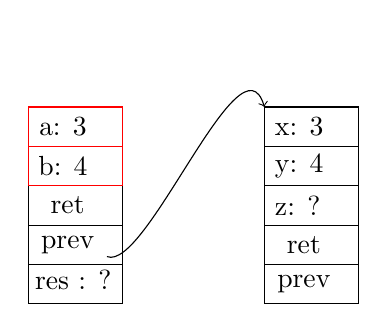
\begin{tikzpicture}
\draw (0,0)  rectangle (1.2,0.5);
\pgftext[at={\pgfpoint{0.65cm}{0.3cm}}]{res : ? } ;

\draw (0,0.5)  rectangle (1.2,1.0);
\pgftext[at={\pgfpoint{0.5cm}{0.75cm}}]{prev} ;
\draw[->] (1.0, 0.6) .. controls (1.5, 0.4) and (2.7, 3.5) .. (3,2.5);


\draw (0,1.0)  rectangle (1.2,1.5);
\pgftext[at={\pgfpoint{0.5cm}{1.25cm}}]{ret} ;

\draw[red] (0,1.5)  rectangle (1.2,2.0);
\pgftext[at={\pgfpoint{0.5cm}{1.75cm}}]{b: 4 } ;

\draw[red] (0,2.0)  rectangle (1.2,2.5);
\pgftext[at={\pgfpoint{0.5cm}{2.25cm}}]{a: 3 } ;

% right one 
\draw (3,0)  rectangle (4.2,0.5);
\pgftext[at={\pgfpoint{3.5cm}{0.25cm}}]{prev} ;

\draw (3,0.5)  rectangle (4.2,1.0);
\pgftext[at={\pgfpoint{3.5cm}{0.75cm}}]{ret} ;

\draw (3,1.0)  rectangle (4.2,1.5);
\pgftext[at={\pgfpoint{3.5cm}{1.25cm}}]{z: ? } ;

\draw (3,1.5)  rectangle (4.2,2.0);
\pgftext[at={\pgfpoint{3.5cm}{1.75cm}}]{y: 4 } ;

\draw (3,2.0)  rectangle (4.2,2.5);
\pgftext[at={\pgfpoint{3.5cm}{2.25cm}}]{x: 3 } ;
\end{tikzpicture}
}
\end{tabular}
\end{tabular}
\begin{itemize}
\item Formal parameters act like local variables in the
activation record of the method.
\item Only difference: they are initialized (with the
value of the actual parameter(s)). 
\item Actual parameters can be arbitrary r-values. 
\end{itemize}

Most common mechanism  (Java, C; default in \Cpp, C\#)
\end{frame}

\begin{frame}[fragile]
\frametitle{Example: Java}
\framesubtitle{Java supports only call-by-value}
%
\vspace*{-0.3cm}
%\begin{java}
\begin{cplus3}
class ConsCell {
    private int head;    
    public ConsCell(int i, ConsCell c) {...}
    ...
    // Mutator, @param h: the new head element
    public void setHead(int h) {
       head = h;
}}
class Try {
    void f() {
       ConsCell x = new ConsCell(1,null);  // x::head = 1
       alter(3,x);                         // x passed by-value 
    }
    void alter(int newHead, ConsCell c) {  
       c.setHead(newHead);                // (*) value of x::head?
}}
\end{cplus3}
%\end{java}

\centerline{
\only<1-2>{\textit{What is the value of \textit{x::head} after (*)\,? 1 or 3?}}
\only<2>{\framebox{\textit{Answer: 3}}}
\only<3>{\textit{In Java, objects are references \ldots}}
\only<4>{\textit{\ldots after copy, $x$ and $c$ reference the same 
 'ConsCell'}}
}
\end{frame}




\begin{frame}[fragile]
\frametitle{}
\framesubtitle{}
\Large{
\begin{center}
Wrong: ``Java implements call-by-reference.''

Right: ``Java implements call-by-value.'' \\
\end{center}
%\begin{center}
{\small Recall reference semantics: if actual parameters are references,
references are copied. 
}
%\end{center}
}
\end{frame}





\begin{frame}[fragile]
\frametitle{Call-by-result}
\framesubtitle{Call-by-copy (2)}
\vspace*{-0.4cm}
\begin{tabular}{ll}
\begin{minipage}{3cm}
\begin{cplus3}
void plus(int a, int b, by-result int c) {
    c = a + b;
}
void f() {
    int x = 3;
    int y = 4; 
    int z;
    plus(x,y,z);
}
\end{cplus3}
\end{minipage}
& 
\begin{tabular}{l}
{\small 
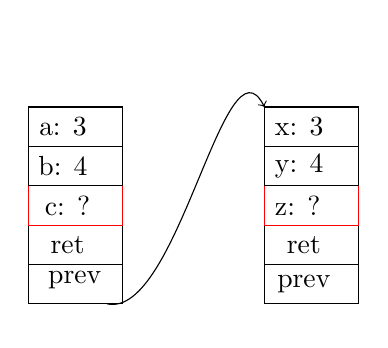
\begin{tikzpicture}
\draw (0,0)  rectangle (1.2,0.5);
\pgftext[at={\pgfpoint{0.65cm}{0.3cm}}]{prev } ;
\draw[->] (1.0, 0.0) .. controls (1.9, -0.2) and (2.5, 3.5) .. (3,2.5);

\draw (0,0.5)  rectangle (1.2,1.0);
\pgftext[at={\pgfpoint{0.5cm}{0.75cm}}]{ret} ;



\draw[red] (0,1.0)  rectangle (1.2,1.5);
\pgftext[at={\pgfpoint{0.5cm}{1.25cm}}]{c: ?} ;

\draw (0,1.5)  rectangle (1.2,2.0);
\pgftext[at={\pgfpoint{0.5cm}{1.75cm}}]{b: 4 } ;

\draw (0,2.0)  rectangle (1.2,2.5);
\pgftext[at={\pgfpoint{0.5cm}{2.25cm}}]{a: 3 } ;

% right one 
\draw (3,0)  rectangle (4.2,0.5);
\pgftext[at={\pgfpoint{3.5cm}{0.25cm}}]{prev} ;

\draw (3,0.5)  rectangle (4.2,1.0);
\pgftext[at={\pgfpoint{3.5cm}{0.75cm}}]{ret} ;

\draw[red] (3,1.0)  rectangle (4.2,1.5);
\pgftext[at={\pgfpoint{3.5cm}{1.25cm}}]{z: ? } ;

\draw (3,1.5)  rectangle (4.2,2.0);
\pgftext[at={\pgfpoint{3.5cm}{1.75cm}}]{y: 4 } ;

\draw (3,2.0)  rectangle (4.2,2.5);
\pgftext[at={\pgfpoint{3.5cm}{2.25cm}}]{x: 3 } ;

\end{tikzpicture}
}
\end{tabular}
\end{tabular}


\begin{itemize}
\item Formal parameters  act like local variables in the
AR of the method. They are not initialized. 
\item Upon return, the value of the formal parameter gets copied
into the actual parameter. 
\item Actual parameters do not have to be initialized (why?), but
must be l-values (why?) 
\end{itemize}
Example: ``out''-parameters in C\# and Ada

\end{frame}

\begin{frame}[fragile]
\frametitle{Example: call-by-result}
\framesubtitle{C\# out parameters}
In C\# 
\begin{itemize}
\item By-result parameters are declared via ``out.'' 
\item The modifier 
is also necessary for the actual argument
(as with ``ref'' parameters).

\begin{cplus3}
void Control (out int x, mytype y)
{
     // x not accessible

     x = process(y);
  
     // now x accessible    
}

int v;
Control(out v);
\end{cplus3}
% Holds the value of process(y)
\end{itemize}
\end{frame}


\begin{frame}[fragile]
\frametitle{Call-by-value-result}
\framesubtitle{Call-by-copy (3)}


\begin{tabular}{ll}
\begin{minipage}{6cm}
\begin{cplus3}
void plus(int a, by-value-result int b) 
{
    b = b + a;
}
void f() {
    int x = 3;
    plus(4,x);
}
\end{cplus3}
\end{minipage}
& 

\begin{tabular}{l}
{\small 
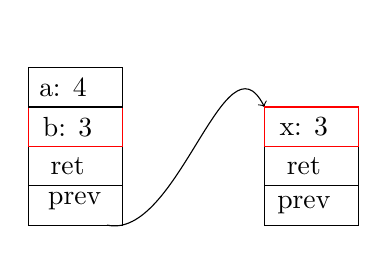
\begin{tikzpicture}
\draw (0,0)  rectangle (1.2,0.5);
\pgftext[at={\pgfpoint{0.65cm}{0.3cm}}]{prev } ;
\draw[->] (1.0, 0.0) .. controls (1.9, -0.2) and (2.5, 2.5) .. (3,1.5);

\draw (0,0.5)  rectangle (1.2,1.0);
\pgftext[at={\pgfpoint{0.5cm}{0.75cm}}]{ret} ;


\draw[red] (0,1.0)  rectangle (1.2,1.5);
\pgftext[at={\pgfpoint{0.5cm}{1.25cm}}]{b: 3} ;

\draw (0,1.5)  rectangle (1.2,2.0);
\pgftext[at={\pgfpoint{0.5cm}{1.75cm}}]{a: 4 } ;



% right one 
\draw (3,0)  rectangle (4.2,0.5);
\pgftext[at={\pgfpoint{3.5cm}{0.25cm}}]{prev} ;

\draw (3,0.5)  rectangle (4.2,1.0);
\pgftext[at={\pgfpoint{3.5cm}{0.75cm}}]{ret} ;

\draw[red] (3,1.0)  rectangle (4.2,1.5);
\pgftext[at={\pgfpoint{3.5cm}{1.25cm}}]{x: 3} ;



\end{tikzpicture}
}
\end{tabular}
\end{tabular}

\begin{itemize}
\item Combination of call-by-value and call-by-result.
\item  Formal parameters are like local variables in the  AR
of the callee.
\item Actual parameters initialize formal parameters; 
at procedure return, the value gets copied back. 
\end{itemize}
Example: Ada ``in-out'' parameters
\end{frame}






\begin{frame}[fragile]
\frametitle{Example: call-by-value-result}
\framesubtitle{``in out'' in Ada}

What gets printed? 4 or 5? 
\visible<2->{\textit{Output: 4}}
\begin{cplus}
type IntegerPair is 
record
   a,b : integer;
end record;

r: IntegerPair; 

procedure sync(s: in out IntegerPair) is
begin
   r.a := r.a + 1;
   s.a := s.a + 1;
end sync;
..
r.a := 3;
sync(r);
put(r.a); --- print 

\end{cplus}
\end{frame}

%\end{document}




\begin{frame}[fragile]
\frametitle{Call-by-value-result vs. call-by-reference}
\framesubtitle{Differences}
Similar, but
\begin{itemize}
\item Different workings  (``operational semantics'')
\begin{itemize}
\item by-value-result: copies objects
\item by-reference: copies addresses only; alias problem
\end{itemize}
\item Different values if actual parameters alias each other.
\begin{cplus}
void p(by-?? int x, by-?? int y) { 
   x++; 
   y++; 
}
int a = 1;
p(a,a);
\end{cplus}
Upon return: 
\begin{itemize}
\item 
Call-by-reference: $a$ has value  3. 
\item 
Call-by-value-result: $a$ has value 2.
\end{itemize}
\end{itemize}
\end{frame}





\begin{frame}[fragile]
\frametitle{Example: C}
\framesubtitle{C supports only call-by-value}
But C has pointers and the address-of operator, which can
achieve the effect of by-reference.


\begin{cplus3}
void plus(int a, int* b) { *b += a;}
void f() {
   int x = 3;
   plus(4,&x);
}
\end{cplus3}
Careful:
\begin{itemize}
\item don't mix  up the C/\cpp address-of operator ``\&'' with
the parameter declarator ``\&'' for reference parameters in \cpp.
\item Address-of is an operator (prefix); the by-reference declarator is postfix.
\end{itemize}
\end{frame}


\begin{frame}[fragile]
\frametitle{Evaluation}
What if the programmer has a choice?
\bigskip

Decision criteria:
\begin{itemize}
\item Correctness first! 
\begin{itemize}
\item \textit{Must} work with copy? Must \textit{not} work with a copy?
\end{itemize}
\item Run-time efficiency
\begin{itemize}
\item Passing parameters: by-reference copies addresses (cheap), by-copy
copies 'objects'
\item Accessing parameters: by-reference incurs indirection, by-copy
gives direct access
\end{itemize}
\item Space-efficiency
\begin{itemize}
\item by-copy requires 2x space
\end{itemize}
\item Safety 
\begin{itemize}
\item by-reference can lead to alias-problems (unless there is
write protection as ``const \&'' in \Cpp)
\end{itemize}
%\item Portability
\end{itemize}



\begin{cplus3}
\end{cplus3}
\end{frame}


\begin{frame}[fragile]
\frametitle{Macro expansion}
\framesubtitle{Danger of name capture}
A \textit{macro} is a named source text fragment. A  processor
replaces the macro name in a program by the corresponding body.
\bigskip 


\begin{itemize}
\item Macros can be used like functions, but aren't functions. Macro
are expanded (substituted) before compilation. 
\item In most languages, macros are unsafe.
\begin{itemize}
\item Exception: hygienic macros (Scheme)
\end{itemize}
\end{itemize}

Standard problem: name capture
\begin{itemize}
\item \textit{Free} variables (X,Y) get bound by local definitions. 
\begin{cplus3}
#define intswap(X,Y) {int temp=X; X=Y; Y=temp;}
int main() {
    int temp=1, b=2;                 
    intswap(temp,b);
    printf(``%d, %d\n'', temp, b);    

}
\end{cplus3}
\end{itemize}
\end{frame}


\begin{frame}[fragile]
\frametitle{Call-by-name}


\begin{tabular}{ll}
\begin{minipage}{4.5cm}
\begin{cplus3}

void f(by-name int a, by-name int b) 
{
    b = 5;
    b = a;
}
int g() {
    int i = 3;
    f(i+1,i);
    return i;
}
\end{cplus3}


\end{minipage}
& 
\begin{tabular}{ll}
{\small 
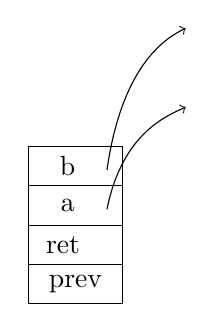
\begin{tikzpicture}

\draw (0,0.5)  rectangle (1.2,1.0);
\pgftext[at={\pgfpoint{0.6cm}{0.75cm}}]{prev} ;

\draw (0,1.0)  rectangle (1.2,1.5);
\pgftext[at={\pgfpoint{0.5cm}{1.25cm}}]{ret } ;

\draw (0,1.5)  rectangle (1.2,2.0);
\pgftext[at={\pgfpoint{0.5cm}{1.75cm}}]{a} ;
\draw[->] (1.0, 1.7) .. controls (1.2, 2.7) and (1.8, 2.9) .. (2,3);

\draw (0,2.0)  rectangle (1.2,2.5);
\pgftext[at={\pgfpoint{0.5cm}{2.25cm}}]{b} ;
\draw[->] (1.0, 2.2) .. controls (1.2, 3.6) and (1.8, 3.9) .. (2,4);

\end{tikzpicture}
}
&
{\small 
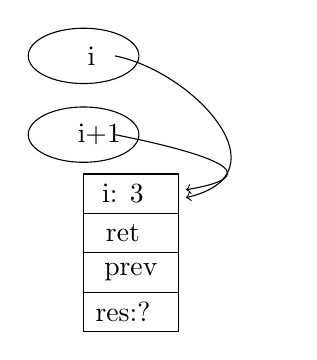
\begin{tikzpicture}
\draw (0,0)  rectangle (1.2,0.5);
\pgftext[at={\pgfpoint{0.5cm}{0.25cm}}]{res:?} ;

\draw (0,0.5)  rectangle (1.2,1.0);
\pgftext[at={\pgfpoint{0.6cm}{0.75cm}}]{prev} ;

\draw (0,1.0)  rectangle (1.2,1.5);
\pgftext[at={\pgfpoint{0.5cm}{1.25cm}}]{ret} ;

\draw (0,1.5)  rectangle (1.2,2.0);
\pgftext[at={\pgfpoint{0.5cm}{1.75cm}}]{i: 3} ;

\draw (0,2.5) ellipse (20pt and 10pt);
\pgftext[at={\pgfpoint{0.2cm}{2.5cm}}]{i+1} ;
\draw[->] (0.4,2.5) .. controls (1.4, 2.3) and (2.5,2.0) .. (1.3,1.8);

\draw (0,3.5) ellipse (20pt and 10pt);
\pgftext[at={\pgfpoint{0.1cm}{3.5cm}}]{i} ;
\draw[->] (0.4,3.5) .. controls (1.4, 3.3) and (2.6,2.0) .. (1.3,1.7);

\end{tikzpicture}
}
\end{tabular}
\end{tabular}

\begin{itemize}
\item Actual parameters evaluated in the context of the caller 
(``closure'').
\item Similar to macro expansion but safe (no name capture). 
\item Each use  of the formal parameter triggers a new
evaluation. 
\item Non-trivial to implement (``thunks''). 
\end{itemize}

 Example : Algol 60, anonymous functions in ML
\bigskip

\end{frame}

\begin{frame}[fragile]
\frametitle{Call-by-need}
Call-by-need can be understood as an optimization of
call-by-name:

\begin{itemize}
\item Actual parameters evaluated in the context of the caller
when they are used the first time.
\item Value is cached; no re-evaluation(``memoization''). 
\end{itemize}

 Example : Haskell

%\begin{tabular}{ll}
%\begin{minipage}{3cm}
\begin{cplus3}

void f(by-n?? int a, by-n?? int b) {
    b = a;
    b = a;
}
int g() {
    int i = 3;
    f(i+1,i);
    return i;
}
\end{cplus3}
Note the difference:
\begin{itemize}
\item In call-by-need, $g$ returns 4.
%\item  
in call-by-name, $g$ returns 5.

\end{itemize}
%\end{minipage}

%\end{tabular}




\end{frame}

\begin{frame}[fragile]
\frametitle{Jensen's device}
\framesubtitle{Call-by-name}
Jensen's device exploits that in call-by-name, a procedure can change the 
value of the variables in its argument; it modifies and re-evaluates
its argument. 

\[
    x = \Sigma_{k=1}^{n} i\cdot v_i
\]
\begin{cplus3}
real procedure Sum (k, lower, upper, vi); 
   value lower, upper;  
   integer k, lower, upper; real vi; 
begin 
   real s; 
   s := 0; 
   for k := lower step 1 until upper do 
      s := s + vi * k; 
   Sum := s 
end;
x := Sum(i,1,10, v[i]);
\end{cplus3}
In the first loop iteration, $v[i]*i$ is evaluated to
$v[1]*1$, in the second to $v[2]*2$, etc. 

\end{frame}


\begin{frame}
\frametitle{Summary}
% Webb, p.382ff.
(In the imperative world, ) 
There are  6 mechanisms for parameter passing. 
\begin{itemize}
\item The behavior of a program depends on the particular parameter-passing
mechanism.
\begin{itemize}
\item Correctness
\item Efficiency
\end{itemize}
\item Program variables are passed: difference reference/value matters
\begin{itemize}
\item Copy of reference variables achieves effects of sharing.
\end{itemize}

\end{itemize}

Other views;
\begin{itemize}
\item In functional programming, the interesting distinction is between
\textit{eager} or \textit{lazy} evaluation of actual parameters. 
\item In declarative languages, parameter passing works entirely
differently (``unification'').
\end{itemize}

\end{frame}


\end{document}

\section{Commands}

\begin{frame}[fragile]
\frametitle{What are commands?}
\framesubtitle{}
Commands are the mechanisms to structure computation in 
imperative and object-oriented (and concurrent) languages:

\begin{itemize}
\item Language constructs that are executed to update
variables 
\item Two classes: statements and expressions
\end{itemize}
Statements
\begin{itemize}
\item No return values; executed because of their side effects 
(i.e., change to the program state).
%XXX
\end{itemize}
Expressions
\begin{itemize}
\item Mathematically and in functional languages:  return a value and produce
no side effects
\item In von-Neumann languages: expressions can have side effects.
\end{itemize}
\end{frame}


\begin{frame}[fragile]
\frametitle{Expressions}
\framesubtitle{}
%Examples
\begin{itemize}
\item Operator expressions: arithmetic, logical, comparison,
sequencing (\texttt{,'} in C/\cpp, \texttt{.} in Smalltalk).

% InC/\cpp evaluated left-to-right; returns: right-most value
% For x=1, y=2: returns 5, leave y at 3  
\begin{cplus3}
x + 1;  x^^6; a && b; mine <= yours; 
// sequencing
  x = ( y +=1, x += y, x+1);
\end{cplus3}
\item Procedure call
\begin{cplus3}
print(a, b);  mul(add(1, 5), mul(3,4));
\end{cplus3}
\item Assignment  (side effect!!)
\begin{cplus3}
x = x + 1;  y +=1;   a = b = c + d; 
\end{cplus3}
\end{itemize}
Evaluation strategy
\begin{itemize}
\item Strict: all operands are evaluated before the operator is applied. 
\item Non-strict: not all operands  are always evaluated when the operator
is applied. 
\end{itemize}
% Show in the example above

\end{frame}

\begin{frame}[fragile]
\frametitle{Strict evaluation}
Strict evaluation results in a bottom-up evaluation of the syntax tree
of an expression. 
\bigskip

Evaluation order of subexpressions
\begin{itemize}
\item does not matter in \textit{pure} programs (= without side
effects);
\item could be specified (e.g., left-to-right),
 but is often left unspecified (why?) and then 
 makes programs with side effects non-portable


\framesubtitle{}
\begin{cplus3}
int x = 1;
int f() {
   return x++;
}
int g(int a, int b) {
   return a+b;
}
int main() {
    printf(``%d\n'', g(x,f()));
    return 0; }   
\end{cplus3}
\end{itemize}
Context of  lambda-calculus/functional programming
\begin{itemize}
\item Applicative-order evaluation/eager evaluation 
\end{itemize}
\end{frame}

\begin{frame}[fragile]
\frametitle{Non-strict evaluation}
\framesubtitle{}
In non-strict evaluation, operands are evaluated when their value
is needed (thus: sometimes not at all). 
Examples:
\begin{itemize}
\item Short-circuit evaluation of boolean expressions
\begin{cplus3}
true or x
-- Ada
if (i <= max_index) and then (a[i] = 0)
\end{cplus3}
\item if-then-else operator (``?'')
\begin{cplus3}
 x ? y : w 
\end{cplus3}
\end{itemize}
Non-strict and strict evaluation have very different effects on
\begin{itemize}
\item termination
\item value
\end{itemize}
Context of  lambda-calculus/functional programming
\begin{itemize}
\item Normal-order evaluation/lazy (delayed) evaluation 
\end{itemize}
\end{frame}



\begin{frame}[fragile]
\frametitle{Statements}
\framesubtitle{}
Programs rarely consist just of a sequence of
assignments. 
%
Classes of (control) statements: 
and for repeating.
\begin{itemize}
\item Selection
\item Iteration
\end{itemize}
%Turing completeness
\bigskip

Control flow:
\begin{itemize}
\item Single-entry, single-exit (``structured programming'')
\begin{itemize}
\item Blocks
\end{itemize}
\item Single-entry, multiple-exit
\begin{itemize}
\item Exit statements; exceptions
\end{itemize}
\item Multiple-entry, multiple-exit
\begin{itemize}
\item Goto statement % (``unstructured programming'')
\end{itemize}
\end{itemize}
\end{frame}

\begin{frame}[fragile]
\frametitle{Selection}
\framesubtitle{}
Selection statements control which path is executed. 
They are either conditional or unconditional. 
\bigskip

Conditional selection statements:
\begin{itemize}
\item 2-way selection
\begin{itemize}
\item If-statement
\end{itemize}

\item N-way selection
\begin{itemize}
\item Case/Switch statement
\end{itemize}

\item Pattern matching in case statements
%
\begin{itemize}
\item Haskell and ML allow pattern matching in the 
\textit{guards} of the case statement; ``_'' (wildcard) marks the default case.
\begin{cplus3}
f x =
    case x of
      0 -> 1
      1 -> 5
      2 -> 2
      _ -> -1
\end{cplus3}
\end{itemize}


\end{itemize}

\end{frame}

\begin{frame}[fragile]\frametitle{Go to in Cobol}

%http://home.swbell.net/mck9/cobol/style/multloop.html
\begin{cplus3}
* Example by Michael C. Kasten
   PERFORM 3900-GET-FIRST-RECORD.
     GO TO 3110-PROCESS-RECORD. -------------------+
     ...                                           |
     GO TO 3100-GET-NEXT-RECORD. -----------+      |
     ...                                    |      |
*                                           |      |
 3100-GET-NEXT-RECORD. <---------------+ <--+      |
*    do some stuff (no GO TOs)         |           |
     GO TO 3110-PROCESS-RECORD. --+    |           |
*                                 |    |           |
 3110-PROCESS-RECORD.  <----------+ <--|-----------+
*    do some other stuff (no GO TOs)   |
     IF NOT END-OF-FILE                |
        GO TO 3100-GET-NEXT-RECORD ----+
     ELSE
        GO TO 3999-EXIT.---------------+
*                                      |
 3999-EXIT.  <-------------------------+
     EXIT.
\end{cplus3}
\end{frame}



\begin{frame}[fragile]\frametitle{Unconditional branching}
\framesubtitle{Goto controversy}
Heated debate in the 60s
\begin{itemize}
\item Boehm \& Jacobi: any goto statement can be transformed into one using
structured control structures (1966)
\item Dijkstra ``Go to statement considered harmful'' (1968)
\begin{itemize}
\item Readability (spaghetti code); correctness
\end{itemize}
\item Knuth:  ``Structured programming with go to Statements'' (1974)
\begin{itemize}
\item Readability; efficiency
\end{itemize}
\end{itemize}

\end{frame}

\begin{frame}[fragile]\frametitle{Go to statements today}
Most languages today use gotos, but in a restricted form: 
\begin{itemize}
\item Ada: no jumps into if-statements and loops or out of
procedures
\item Java: no \texttt{goto} (reserved word) But: labeled
 statements (break and continue) for controlled jumps

\item C\#: restricted to labels in the scope
and cases in a switch-statement
%http://msdn2.microsoft.com/en-us/library/13940fs2(VS.71).aspx
\begin{cplus3}
{
      string myNumber = Console.ReadLine();
      // Search:
      for (int i = 0; i < x; i++)
         for (int j = 0; j < y; j++)
            if (myArray[i,j].Equals(myNumber))
               goto Found;
      Console.WriteLine("Number {0}  not found.", myNumber);
      goto Finish;
   Found:
      Console.WriteLine("Number {0}  found.", myNumber);
   Finish: 
      Console.WriteLine("End of search.");
}
\end{cplus3}
\end{itemize}
\end{frame}

\begin{frame}[fragile]
\frametitle{Iteration}
\framesubtitle{Loops}
%Watt, p.82

Indefinite iterations:
\begin{itemize}
\item Number of iterations not fixed
\item Loop logically controlled (predicates)
\begin{cplus3}
while (C) E  ==   if (C) then {
                      E
                      while (C) E
                  }
\end{cplus3}
\end{itemize}
Definite iterations:
\begin{itemize}
\item Number of iterations fixed 
\item Loop controlled by counter 
\begin{cplus3}
// Java
for (Date date : dates)
   System.out.println(date);
// C#
String[] breakfast = {``coffee'', ``milk'', ``newspaper'');
foreach(String item in breakfast)
   Console.WriteLine(``Name: {0}'', name);
\end{cplus3}
\end{itemize}

\end{frame}


\begin{frame}[fragile]
\frametitle{Iterators}
\framesubtitle{}
Iterators are pervasive in object-oriented programming, but their
functionality and purpose varies greatly. 

\begin{itemize}
\item CLU

\url{http://www.lcs.mit.edu/publications/pubs/pdf/MIT-LCS-TR-561.pdf}
\begin{java}
// 
produces all the elements in set s, but it yields them one at a time. 
elements = iter (s: set[t]) yields (t)

// An iterator is called in a for statement:
for x: int in set[int]$elements(coll) do
\end{java}
\item Java XXX
\item \Cpp/Standard Template Library
\begin{itemize}
\item Minimal traversal requirements (generic programming) XXX
\end{itemize}
\end{itemize}
\end{frame}
\end{document}

